% Drawing 81/01-2 -- folder 81, batch 01, archive page 11 (PDF page 12).
% Transcription: feuillet de dessins de la même famille que la page 9 : disques coupés de cordes, une région triangulaire ou quadrangulaire hachurée, trois marqués « OK », des variantes introduites par « ou » ; sous eux les graphes : un triangle, un point, un tripode épais en « Y », un carré, un triangle surmonté d'un segment, un rectangle coupé d'une diagonale, un triangle à point intérieur. À droite, deux axes fléchés en équerre et, dans l'angle, des courbes qui se croisent et deux disques coupés d'arcs
% Kind: page of disks cut by chords, with their graphs, and crossing curves. Method 2 (schematic redraw from the facsimile). Status: partial.
% Notes: Whole sheet. Redrawn schematically: the four large disks of the top row (hatched regions, "OK" marks, the variants introduced by "ou" with their small disks), the row of graphs (triangle, point, the thick tripod Y, square, triangle with a segment), the disks and hatched disk at the left (with "OK" and the variants), the rectangle with a diagonal and the triangle with an inner point; on the right, the two arrowed axes at right angles and in the corner the crossing curves and the two disks cut by arcs. The struck scribbles (a "b"-like sign under the second disk, a zigzag) are left out. Positions are approximate, and the crossing curves of the right part are simplified.
% Coordinates: 1 unit = 1 mm = 1/100 of the crop width (bbox in page fractions: [0.1, 0.06, 0.95, 0.48]).
% Redrawn by Claude (claude-opus-5-5), issue #73, 2026-11-07; not checked by a human; not compiled (no TeX in the session).
% Rights: reproduces part of the work -- behind RENDER_TRANSCRIPTS, never published by itself.
\documentclass[tikz,border=3pt]{standalone}
\usepackage{amsmath,amssymb}
\usetikzlibrary{patterns,arrows.meta}
\tikzset{pencil/.style={black!45}, struck/.style={black!35}, mark/.style={circle,draw,inner sep=1.3pt}, pt/.style={circle,fill,inner sep=0.9pt}, opt/.style={circle,draw,fill=white,inner sep=1.1pt}}
\begin{document}
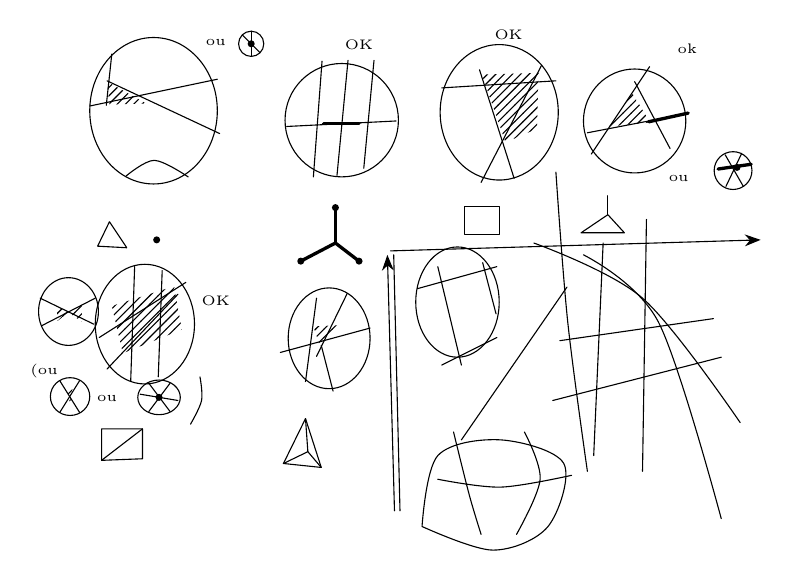
\begin{tikzpicture}[x=1mm,y=1mm,line cap=round,line join=round,font=\scriptsize]
\draw (15.9,-13.2) ellipse[x radius=8.1, y radius=9.3];
\draw (7.8,-12.6) -- (24,-9.2);
\draw (10,-9.4) -- (24.3,-16.1);
\draw (10.6,-6) -- (9.9,-12.5);
\fill[pattern=north east lines] (10,-9.5) -- (10.3,-12.4) -- (15,-12.3) -- cycle;
\draw plot[smooth, tension=0.55] coordinates {(12.4,-21.5) (16,-19.5) (20.3,-21.6)};
\node[inner sep=1pt] at (23.8,-4.5) {\tiny ou};
\draw (28.3,-4.7) circle[radius=1.6];
\draw (27.2,-3.6) -- (29.4,-5.8);
\draw (28.3,-3.1) -- (28.3,-6.3);
\node[pt] at (28.3,-4.7) {};
\draw (39.8,-14.4) ellipse[x radius=7.2, y radius=7.2];
\draw (37.3,-6.9) -- (36.2,-21.6);
\draw (40.6,-6.8) -- (39.2,-21.4);
\draw (43.9,-6.8) -- (42.6,-20.5);
\draw (32.8,-15.2) -- (46.7,-14.5);
\draw[very thick] (37.5,-14.8) -- (42,-14.8);
\node[inner sep=1pt] at (42,-4.8) {\tiny OK};
\draw (59.8,-13.4) ellipse[x radius=7.5, y radius=8.6];
\draw (57.3,-8) -- (61.7,-21.8);
\draw (65.2,-7.4) -- (57.5,-22.3);
\draw (52.5,-10.3) -- (67,-9.4);
\fill[pattern=north east lines] (57.6,-8.6) -- (64.8,-8.4) -- (64.6,-15.5) -- (60.6,-17.2) -- cycle;
\node[inner sep=1pt] at (61,-3.6) {\tiny OK};
\draw (77,-14.5) ellipse[x radius=6.5, y radius=6.6];
\draw (71,-16) -- (83.5,-13.6);
\draw (71.5,-18.7) -- (78.9,-7.6);
\draw (77,-9.5) -- (81.5,-18);
\fill[pattern=north east lines] (73.7,-15.2) -- (76.7,-11) -- (79,-14.7) -- cycle;
\draw[very thick] (78.8,-14.6) -- (83.8,-13.5);
\node[inner sep=1pt] at (83.7,-5.3) {\tiny ok};
\node[inner sep=1pt] at (82.6,-21.8) {\tiny ou};
\draw (89.5,-20.8) circle[radius=2.4];
\draw[very thick] (87.6,-20.6) -- (91.8,-20);
\draw (88.5,-18.8) -- (90.8,-22.8);
\draw (90.6,-18.6) -- (88.6,-22.8);
\node[pt] at (90,-20.4) {};
\draw (8.8,-30.4) -- (10.3,-27.3) -- (12.5,-30.6) -- cycle;
\node[pt] at (16.3,-29.6) {};
\draw[very thick] (39,-30) -- (39,-25.5);
\draw[very thick] (39,-30) -- (34.6,-32.3);
\draw[very thick] (39,-30) -- (42,-32.3);
\node[pt] at (39,-25.5) {};
\node[pt] at (34.6,-32.3) {};
\node[pt] at (42,-32.3) {};
\draw (55.4,-25.4) -- (59.8,-25.4) -- (59.8,-28.9) -- (55.4,-28.9) -- cycle;
\draw (70.2,-28.7) -- (75.7,-28.7) -- (73.6,-26.4) -- cycle;
\draw (73.6,-26.4) -- (73.6,-24);
\draw (5.1,-38.7) ellipse[x radius=3.8, y radius=4.3];
\draw (1.5,-37) -- (8.3,-40.3);
\draw (1.7,-40.5) -- (8.5,-37);
\fill[pattern=north east lines] (3.6,-38) -- (5.1,-38.8) -- (3.7,-39.9) -- cycle;
\fill[pattern=north east lines] (5.1,-38.8) -- (6.8,-37.8) -- (6.8,-40) -- cycle;
\draw (14.8,-40.3) ellipse[x radius=6.3, y radius=7.6];
\fill[pattern=north east lines] (10.6,-38) -- (18.5,-35.5) -- (19.5,-41) -- (12,-44) -- cycle;
\draw (9,-42) -- (20,-35);
\draw (10,-46) -- (19,-36.5);
\draw (13.5,-33) -- (13,-47.5);
\draw (17,-33.5) -- (16.5,-47);
\node[inner sep=1pt] at (23.8,-37.3) {\tiny OK};
\node[inner sep=1pt] at (2,-46.3) {\tiny (ou};
\draw (5.3,-49.5) ellipse[x radius=2.5, y radius=2.4];
\draw (4,-47.5) -- (6.5,-51.5);
\draw (6.5,-47.5) -- (4,-51.5);
\fill[pattern=north east lines] (4.9,-48.5) -- (5.6,-48.5) -- (5.3,-50.4) -- cycle;
\node[inner sep=1pt] at (10,-49.7) {\tiny ou};
\draw (16.6,-49.6) ellipse[x radius=2.7, y radius=2.2];
\draw (14.2,-49.2) -- (19,-50);
\draw (15.3,-47.8) -- (18,-51.4);
\draw (18,-47.8) -- (15.3,-51.4);
\node[pt] at (16.6,-49.6) {};
\draw plot[smooth, tension=0.55] coordinates {(21.8,-47) (22,-50) (20.6,-53)};
\draw (9.3,-53.6) -- (14.5,-53.6) -- (14.5,-57.4) -- (9.3,-57.6) -- cycle;
\draw (9.3,-57.6) -- (14.5,-53.6);
\draw (32.4,-58) -- (35.2,-52.3) -- (37.2,-58.5) -- cycle;
\draw (35.5,-56.5) -- (32.4,-58);
\draw (35.5,-56.5) -- (35.2,-52.3);
\draw (35.5,-56.5) -- (37.2,-58.5);
\draw (38.2,-42.1) ellipse[x radius=5.2, y radius=6.4];
\draw (32,-43.9) -- (43.4,-40.8);
\draw (36.6,-37) -- (35.2,-47.6);
\draw (40.5,-36.4) -- (36.6,-44.4);
\draw (37.2,-43) -- (38.7,-48.8);
\fill[pattern=north east lines] (36.2,-40.6) -- (40,-40.4) -- (37,-43) -- cycle;
\draw[-{Stealth[length=2mm]}] (46,-31) -- (93,-29.6);
\draw[-{Stealth[length=2mm]}] (46.5,-64) -- (45.6,-31.5);
\draw (47.2,-64) -- (46.4,-31.5);
\draw (54.5,-37.5) ellipse[x radius=5.3, y radius=7];
\draw (49.4,-35.8) -- (59.5,-33);
\draw (52,-33) -- (55,-45.5);
\draw (57.7,-32.5) -- (59.4,-39);
\draw (52.5,-45.5) -- (59.5,-42);
\draw plot[smooth, tension=0.55] coordinates {(50,-66) (52,-57) (60,-55) (68,-58) (66,-66) (59,-69) (50,-66)};
\draw plot[smooth, tension=0.55] coordinates {(52,-60) (60,-61) (69,-59.5)};
\draw plot[smooth, tension=0.55] coordinates {(54,-54) (56,-62) (57.5,-67)};
\draw plot[smooth, tension=0.55] coordinates {(63,-54) (65,-60) (62,-67)};
\draw plot[smooth, tension=0.55] coordinates {(67,-21) (68.5,-40) (71,-59)};
\draw (68.4,-35.6) -- (55,-55);
\draw plot[smooth, tension=0.55] coordinates {(64.2,-30) (78,-37) (90.4,-52.8)};
\draw (67.5,-42.4) -- (87,-39.6);
\draw (66.6,-50) -- (88,-44.5);
\draw (73,-30) -- (71.8,-57);
\draw (78.5,-27) -- (78,-59);
\draw plot[smooth, tension=0.55] coordinates {(70.5,-31.5) (80,-40) (88,-65)};
\end{tikzpicture}
\end{document}
